\documentclass{article}
\usepackage[french]{babel}
\usepackage[utf8]{inputenc}
\usepackage[a4paper, total={6in, 9in}]{geometry}
\usepackage{authblk}
\usepackage{graphicx}
\graphicspath{{./imgs/}}
%Titre
\title{Rapport Skyscraper}
\author{Oriane RENARD, Alexandre L'HUMEAU}\affil{Département informatique - Paris 8}
\date{2022}
%Début doc
\begin{document}
\maketitle
\topskip0pt
\vspace*{\fill}
\tableofcontents
\vspace*{\fill}
\newpage
\section{Le skyscraper}
\subsection{But du jeu}
L'objectif est de placer un gratte-ciel dans chacune des cellules en suivant ces règles :
- La taille du skyscraper va de 1 à la taille de la grille, ex: 1 à 4 pour une taille de 4
\begin{center}
	
\includegraphics{taille_grille.png}
\end{center}
- Vous ne pouvez pas avoir deux immeubles de la même taille dans la même ligne ou colonne
\begin{center}
	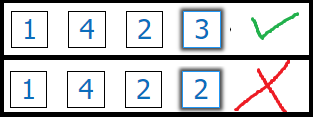
\includegraphics{lignevalide.png}
\end{center}
- Les nombres sur les cotés de la grille indique le nombre de gratte-ciel visibles depuis la position.
\\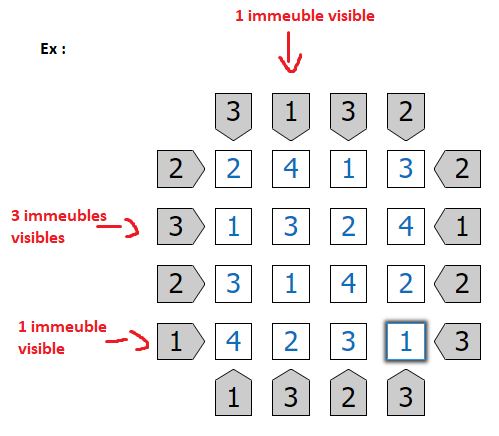
\includegraphics{immeubles_vis.png}\\
\subsection{Les données}
Les données qui sont mises à disposition sont:
- des paires de chiffres définissant les immeubles visibles qu'on va représenter par une liste de tuples.
- une matrice représentant les immeubles et leurs tailles, qu'on va représenter par une liste d'entiers.
\subsection{Étapes de résolution}
L'objectif va être d'abord de vérifier que les données fournies sont valides, après quoi on va
lire les lignes et sortir l'ensemble des lignes valides, après quoi on va vérifier que les colonnes sont valides,
si les lignes et les colonnes sont valides le skyscraper est résolu.
\section{Prédicats}
Pour résoudre ce problème nous avons diviser les prédicats en 4 parties distinctes.
\subsection{Vérifications}
Tout d'abord les prédicats de vérification, ils nous ont servi à vérifier que les éléments fournis au démarrage 
soient bien formattés et du bon type.
\begin{center}
\end{center}
\subsection{Résolution de ligne}
\subsection{Résolution de lignes}
\subsection{Résolution de colonnes}
\subsection{Affichage}
\section{Résultat}
\subsection{Limitations}
\subsection{Exécution}

\end{document}